\documentclass[sigconf,nonacm]{acmart}

\usepackage[utf8]{inputenc}
\usepackage[T1]{fontenc}
\usepackage{graphicx}
\usepackage{booktabs}
\usepackage{amsmath}
\usepackage{microtype}
\usepackage{subcaption}

\bibliographystyle{ACM-Reference-Format}

\begin{document}

\title{TA3 – Transformação Perspectiva}

\author{Luan de Oliveira Magalhães}
\email{luan3642@hotmail.com}
\affiliation{%
  \institution{Departamento de Informática\\Universidade Federal do Paraná}
  \city{Curitiba}
  \state{Paraná}
  \country{Brasil}}

\author{Raul José Silvério da Silva}
\email{raul.silverio@ufpr.br}
\orcid{0009-0006-5091-1584}
\affiliation{%
  \institution{Departamento de Informática\\Universidade Federal do Paraná}
  \city{Curitiba}
  \state{Paraná}
  \country{Brasil}}

\author{Vinícius Lázaro Bartolomeu}
\email{vinicius.bartolomeu@ufpr.br}
\affiliation{%
  \institution{Departamento de Informática\\Universidade Federal do Paraná}
  \city{Curitiba}
  \state{Paraná}
  \country{Brasil}}

\begin{abstract}
    Este trabalho apresenta a resolução da terceira tarefa do projeto de Visão Computacional e Percepção, que consiste na implementação de uma transformação de perspectiva utilizando a biblioteca OpenCV. A tarefa envolve a manipulação de imagens para criar um efeito de perspectiva, permitindo a visualização de objetos em diferentes ângulos. O trabalho inclui a descrição do processo de transformação, a implementação do código e a análise dos resultados obtidos.
\end{abstract}

\keywords{Visão Computacional, Transformação Perspectiva, Homografia, OpenCV, Mapa de projeção plana}

\maketitle


%--------------------------------------------------------------------
\section{Transformação de Perspectiva}
A transformação de perspectiva é uma técnica fundamental em visão computacional, permitindo a manipulação e a análise de imagens de diferentes ângulos e pontos de vista. Essa técnica é especialmente útil em aplicações como realidade aumentada, robótica e reconstrução 3D.

A transformação de perspectiva pode ser descrita matematicamente por meio de matrizes. Dada uma imagem e um conjunto de pontos de origem e destino, podemos calcular a matriz de transformação que mapeia os pontos da imagem original para a nova perspectiva desejada.
A matriz de transformação é uma matriz 3x3 que pode ser representada como:

\[
H = \begin{pmatrix}
h_{11} & h_{12} & h_{13} \\
h_{21} & h_{22} & h_{23} \\
h_{31} & h_{32} & h_{33}
\end{pmatrix}
\]

onde \(h_{ij}\) são os coeficientes da matriz de homografia. 
A transformação de perspectiva é aplicada a um ponto \((x, y)\) na imagem original para obter o ponto transformado \((x', y')\) na nova imagem, utilizando a seguinte equação:
\[
\begin{pmatrix}
x' \\
y' \\ 1
\end{pmatrix}
=
H \cdot
\begin{pmatrix}
x \\
y \\ 1
\end{pmatrix}
\]
onde \((x', y')\) são as coordenadas do ponto transformado e \((x, y)\) são as coordenadas do ponto original.

%--------------------------------------------------------------------

\section{Método}
A implementação da transformação de perspectiva foi realizada utilizando a biblioteca OpenCV, que fornece funções eficientes para manipulação de imagens e aplicação de transformações geométricas. O processo envolveu os seguintes passos:
\begin{enumerate}
    \item Carregamento da imagem original.
    \item Definição dos pontos de origem e destino para a transformação de perspectiva.
    \item Cálculo da matriz utilizando a função \texttt{cv2.getPerspectiveTransform()}.
    \item Aplicação da transformação utilizando a função \texttt{cv2.warpPerspective()}.
    \item Exibição da imagem resultante.
\end{enumerate}


O código implementado está disponível no repositório do projeto, disponível em \url{https://github.com/silveriorj/transformacao-perspectiva} \cite{github_ta03_repository}.

A seguir, apresentamos um exemplo de código que ilustra a implementação da transformação de perspectiva:


\begin{verbatim}
import cv2
import numpy as np

def transform_perspective(
  image, 
  src_points, 
  dst_points, 
  output_size
  ):
    """
    Transforms the perspective of an image using OpenCV.

    :param image: Input image as a NumPy array.
    :param src_points: List of four points (x, y)
    :param dst_points: List of four points (x, y)
    :param output_size: Tuple (width, height)
    :return: Perspective-transformed image.
    """
    # Compute the perspective transformation matrix
    matrix = cv2.getPerspectiveTransform(
      np.float32(src_points), 
      np.float32(dst_points)
    )
    
    # return the perspective transformation
    return cv2.warpPerspective(
      image, 
      matrix, 
      output_size
    )
\end{verbatim}


%--------------------------------------------------------------------

\section{Resultados}
A transformação de perspectiva foi aplicada a uma imagem de exemplo, resultando em uma nova imagem com a perspectiva alterada.

\begin{figure}[H]
  \centering
  \begin{subfigure}[b]{0.45\linewidth}
    \centering
    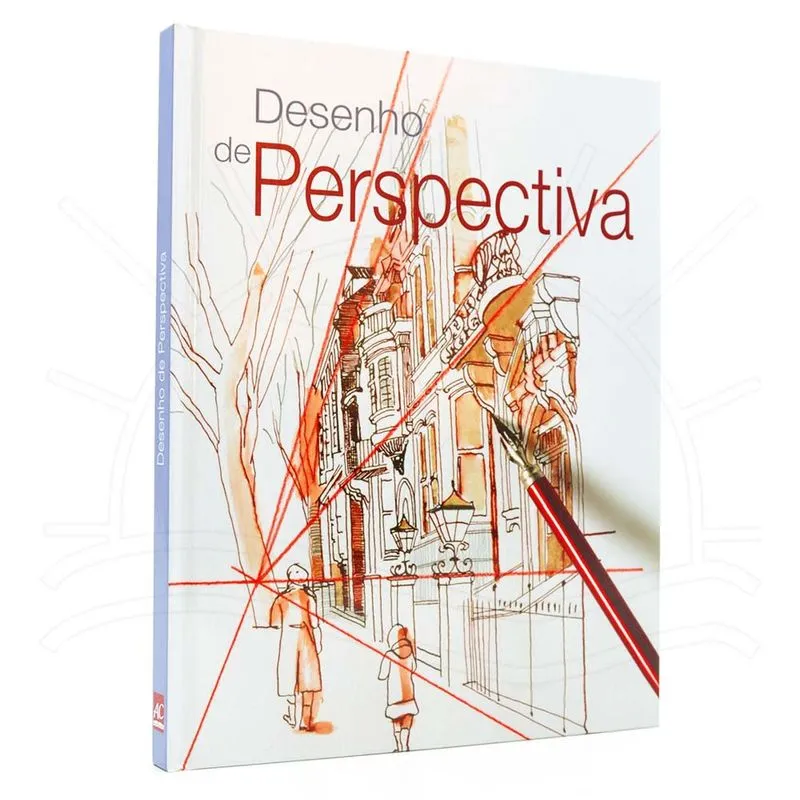
\includegraphics[width=\linewidth]{resources/input1.jpg}
    \caption{Imagem original}
    \Description{Imagem original capturada em um ângulo reto.}
    \label{fig:one}
  \end{subfigure}
  \hfill
  \begin{subfigure}[b]{0.45\linewidth}
    \centering
    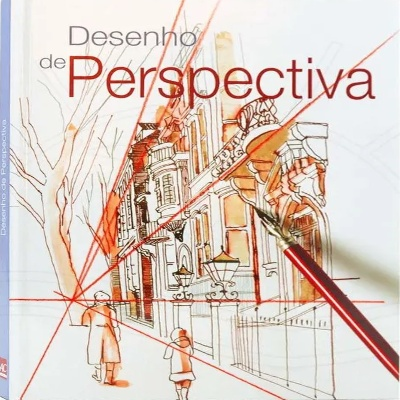
\includegraphics[width=\linewidth]{resources/output1.jpg}
    \caption{Imagem transformada}
    \Description{Imagem transformada com uma perspectiva inclinada.}
    \label{fig:two}
  \end{subfigure}

  \centering
  \begin{subfigure}[b]{0.45\linewidth}
    \centering
    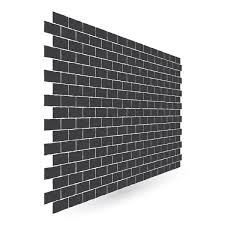
\includegraphics[width=\linewidth]{resources/input2.jpg}
    \caption{Imagem original}
    \Description{Imagem original capturada em um ângulo reto.}
    \label{fig:three}
  \end{subfigure}
  \hfill
  \begin{subfigure}[b]{0.45\linewidth}
    \centering
    
\includegraphics[width=\linewidth]{resources/output2.jpg}
    \caption{Imagem transformada}
    \Description{Imagem transformada com uma perspectiva inclinada.}
    \label{fig:four}
  \end{subfigure}
  \caption{Comparação entre a imagem original e a imagem transformada.}
  \label{fig:resultados}
\end{figure}


A figura \ref{fig:resultados} mostra a imagem original e a imagem transformada. A imagem original foi capturada em um ângulo inclinado, enquanto a imagem transformada apresenta uma perspectiva em angulo reto, demonstrando a eficácia da transformação aplicada.


%--------------------------------------------------------------------


\section{Conclusão}


\bibliography{references}

\end{document}
